
\section{Stakeholders and Requirements}
\label{sect:require}

\subsection{Stakeholders}

\begin{center}
\begin{longtable}{|p{3cm}|p{6.6cm}|p{2cm}|}
\hline \multicolumn{1}{|p{3cm}|}{\textbf{ID (Stakeholder)}} & \multicolumn{1}{|p{6.6cm}|}{\textbf{Description (how they impact the product and/or development process)}} & \multicolumn{1}{|p{2cm}|}{\textbf{Priority}} \\ \hline 
\endfirsthead

\multicolumn{3}{c}%
{{\bfseries \tablename\ \thetable{} -- continued from previous page}} \\
\hline \multicolumn{1}{|p{3cm}|}{\textbf{ID (Stakeholder)}} &
\multicolumn{1}{|p{6.6cm}|}{\textbf{Description (how they impact the product and/or development process)}} &
\multicolumn{1}{|p{2cm}|}{\textbf{Priority}} \\ \hline 
\endhead

\hline
\endlastfoot


Owner & An individual or company that owns the food truck business that intend to serve food to customers and make a profit from the sale. They understand how the food truck should operate and will provide features that can be implemented to make specific processes more efficient & High \\\hline
Manager & An individual who is in charge of the employees and the facilities they work in & High \\\hline
Chef & Person who will prepare and cook food in the kitchen and the food truck based on the menu items established & High \\\hline
Employees & Individuals who work for the food truck business. They may interact with customers to sell food, take orders, process these orders and help prepare food & High \\\hline
Developer & An individual or group that will build and update an application that will be used by the food truck staff and potentially other members. & High \\\hline
Suppliers & Provides products and goods ordered from the business to maintain the stock required for further sales & Low \\\hline
Banks & Handles the finances of the business and also offer other financial benefits & Low \\\hline
General Customer & Potential customers interested in the what the food truck has to offer and possibly buy items & Medium \\\hline
Tourists & Same as a general customer but may speak other languages. Also be able to order and view items but have in a language that is easy for them to understand & Medium \\\hline
Event Organisers & People or companies that can potentially hire a food truck business to cater food for the people attending the organised event & Low \\
\end{longtable}
\end{center}
\newpage
\subsection{Use Case Diagrams}
\begin{figure}[!htb]
	\centering
	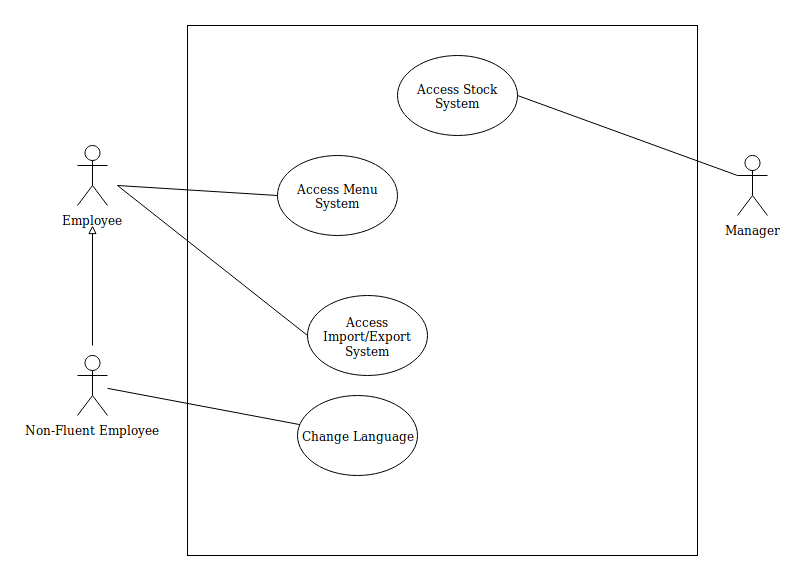
\includegraphics[width=0.7\textwidth]{main_case}
	\caption{Main Use Case}
	\label{fig:maincase}
\end{figure}
\begin{figure}[!htb]
	\centering
	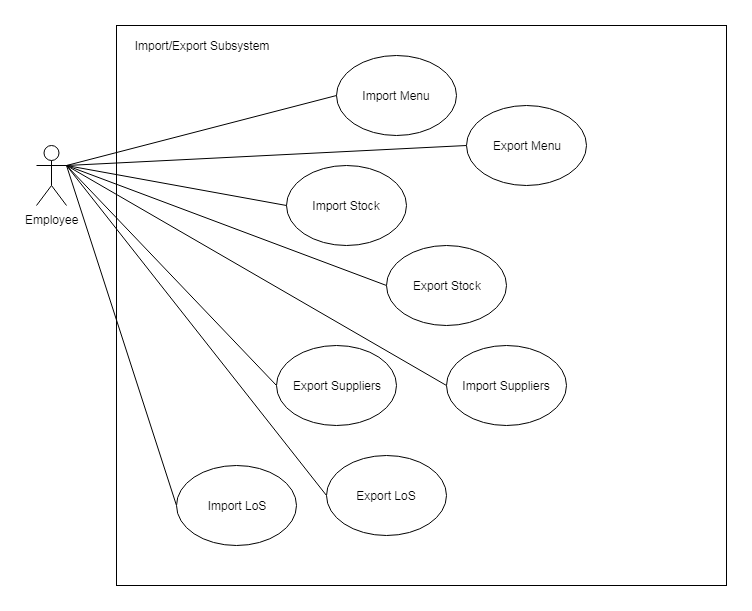
\includegraphics[width=0.7\textwidth]{import_export_case}
	\caption{Import/Export Case}
	\label{fig:iocase}
\end{figure}
\begin{figure}[!htb]
	\centering
	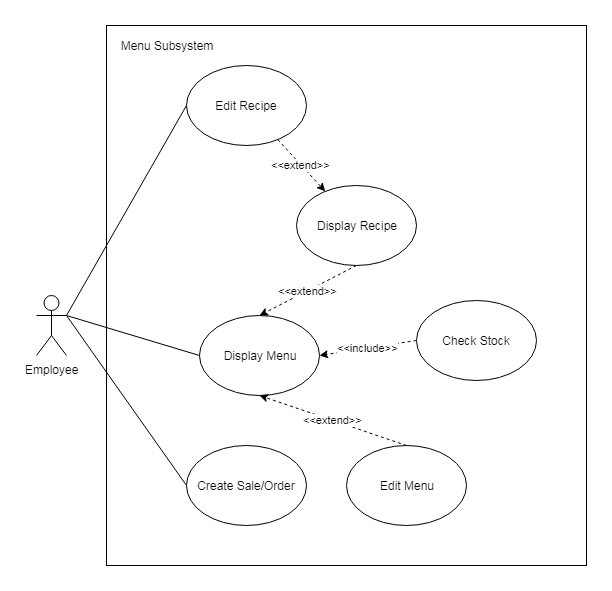
\includegraphics[width=0.7\textwidth]{menu_case}
	\caption{Menu Use Case}
	\label{fig:menucase}
\end{figure}
\begin{figure}[!htb]
	\centering
	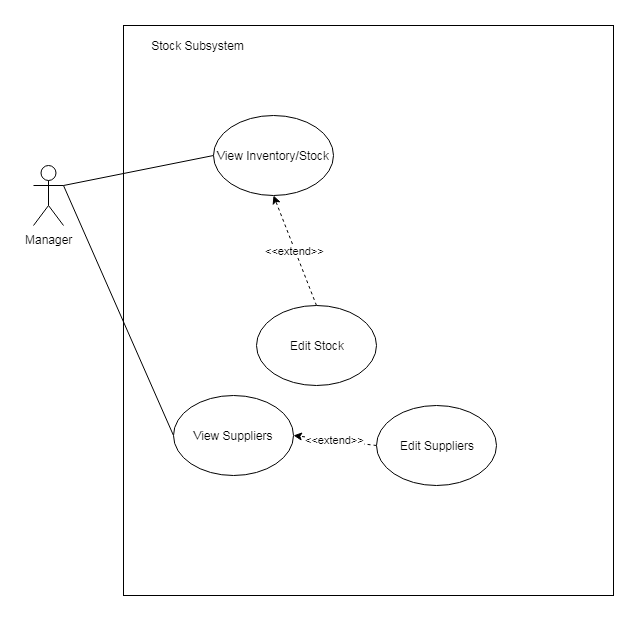
\includegraphics[width=0.7\textwidth]{stock_case}
	\caption{Stock Use Case}
	\label{fig:stockcase}
\end{figure}
\newgeometry{margin=2cm}
\begin{landscape}
\subsection{Textual Use Cases}
\begin{longtable}{|p{.04\textwidth}|p{.11\textwidth}|p{.05\textwidth}|p{.1\textwidth}|p{.25\textwidth}|p{.25\textwidth}|p{.1\textwidth}|}
	\hline \multicolumn{1}{|p{.04\textwidth}}{\textbf{ID}} & \multicolumn{1}{|p{.11\textwidth}}{\textbf{Name}} & \multicolumn{1}{|p{.05\textwidth}}{\textbf{Actor}} & \multicolumn{1}{|p{.1\textwidth}}{\textbf{Pre conditions}} & \multicolumn{1}{|p{.25\textwidth}}{\textbf{Basic Flow}} & \multicolumn{1}{|p{.25\textwidth}}{\textbf{Exceptional Flow}} & \multicolumn{1}{|p{.1\textwidth}|}{\textbf{Post Conditions}}\\ \hline 
	\endfirsthead
	
	\multicolumn{3}{c}%
	{{\bfseries \tablename\ \thetable{} -- continued from previous page}} \\
	\hline \multicolumn{1}{|p{.04\textwidth}}{\textbf{ID}} & \multicolumn{1}{|p{.11\textwidth}}{\textbf{Name}} & \multicolumn{1}{|p{.05\textwidth}}{\textbf{Actor}} & \multicolumn{1}{|p{.1\textwidth}}{\textbf{Pre conditions}} & \multicolumn{1}{|p{.25\textwidth}}{\textbf{Basic Flow}} & \multicolumn{1}{|p{.25\textwidth}}{\textbf{Exceptional Flow}} & \multicolumn{1}{|p{.1\textwidth}|}{\textbf{Post Conditions}}\\ \hline 
	\endhead
	
	\hline
	\endlastfoot
	
	\rownumber & Display Recipes & Employee & Recipe exists & 
	\begin{enumerate}[wide, labelwidth=!, labelindent=0pt, nosep, topsep=0pt, parsep=0pt]
		\item User clicks on the display recipe button
		\item The screen shows a list of ingredients in each recipe and the required amount of each ingredient
		\item User clicks return button to return to the previous screen
	\end{enumerate} & If no recipes exist:\begin{enumerate}[wide, labelwidth=!, labelindent=0pt, nosep, topsep=0pt, parsep=0pt]
		\item User clicks on the display recipe button
		\item The screen shows an error saying that no recipe exists
		\item User clicks return button to return to the previous screen
	\end{enumerate} & \\\hline

	 \rownumber & Edit Recipes & Employee & Recipe exists & 
	\begin{enumerate}[wide, labelwidth=!, labelindent=0pt, nosep, topsep=0pt, parsep=0pt]
		\item User clicks on the edit recipe button
		\item The screen shows a data input screen
		\item The user may change the name, ingredients, and amount of ingredient in recipe
		\item The user clicks a save recipe button
		\item The user is returned to the previous screen
	\end{enumerate} & If no recipes exist:\begin{enumerate}[wide, labelwidth=!, labelindent=0pt, nosep, topsep=0pt, parsep=0pt]
		\item User clicks on the edit recipe button
		\item The screen shows a data input screen
		\item The user inputs a recipe name
		\item The user enters the ingredients needed and the required amount
		\item The user clicks a save recipe button
		\item The user is returned to the previous screen
	\end{enumerate} & \\\hline

	 \rownumber & Display Menu & Employee & Menu exists & 
	\begin{enumerate}[wide, labelwidth=!, labelindent=0pt, nosep, topsep=0pt, parsep=0pt]
		\item User clicks on the display menu button
		\item The screen shows the menu as a list of recipes
		\item User clicks return button to return to the previous screen
	\end{enumerate} & If no recipes exist:\begin{enumerate}[wide, labelwidth=!, labelindent=0pt, nosep, topsep=0pt, parsep=0pt]
		\item User clicks on the display menu button
		\item The screen shows an error saying that no menu exists
		\item User clicks return button to return to the previous screen
	\end{enumerate} & \\\hline

	 \rownumber & Edit Menu & Employee & Menu exists & 
	\begin{enumerate}[wide, labelwidth=!, labelindent=0pt, nosep, topsep=0pt, parsep=0pt]
		\item User clicks on the edit menu button
		\item The screen shows the menu editor screen
		\item The user can then add and remove recipes from the menu
		\item User clicks return button to return to the previous screen
	\end{enumerate} & If no recipes exist:\begin{enumerate}[wide, labelwidth=!, labelindent=0pt, nosep, topsep=0pt, parsep=0pt]
		\item User clicks on the edit menu button
		\item The screen shows an error saying that no menu exists
		\item User clicks return button to return to the previous screen
	\end{enumerate} & \\\hline

\end{longtable}
\end{landscape}
\restoregeometry

